
\chapter{Localisation}

This chapter focuses on robot localisation in a simulated environment, achieved through the computation of its position and orientation using wheel encoder readings, a method known as odometry. The robot calculates the distance traveled by each wheel, determining the forward movement as:

\[
\Delta_{\text{center}} = \frac{\Delta_{\text{left}} + \Delta_{\text{right}}}{2}
\]

and the change in orientation as:

\[
\Delta_{\theta} = \frac{\Delta_{\text{right}} - \Delta_{\text{left}}}{\text{wheel base}}
\]

Using these values, the robot updates its global position and orientation at each step of the simulation. The updated coordinates are given by:

\[
x_{\text{new}} = x_{\text{old}} + \Delta_{\text{center}} \cdot \cos(\theta_{\text{old}})
\]

\[
y_{\text{new}} = y_{\text{old}} + \Delta_{\text{center}} \cdot \sin(\theta_{\text{old}})
\]

\[
\theta_{\text{new}} = \theta_{\text{old}} + \Delta_{\theta}
\]

The system continuously monitors the encoder values during each simulation step, ensuring real-time refinement of the robot's position and orientation. By leveraging these calculations, the robot maintains an accurate understanding of its location within the environment, which is essential for precise movement and navigation.

\paragraph*{}
In this project, we initially set out to implement SLAM for the TurtleBot3 in the Webots simulation environment, but later realized that our implementation was limited to localization on a predetermined map rather than full SLAM. The TurtleBot3 was configured with motors for continuous movement, enabling exploration and data collection, and equipped with a LIDAR sensor for 360° obstacle detection. Encoders tracked wheel rotations, and odometry calculations used differential drive kinematics to update the robot's position and orientation. Localization was achieved by updating the robot’s position based on encoder data and interpreting LIDAR data relative to a predefined rectangular map with fixed dimensions. This predefined knowledge of the environment meant that the implementation did not fully achieve SLAM, which requires both simultaneous mapping and localization in an unknown environment. The robot updated its position and visualized its progress on the predetermined map in real-time, with periodic visualizations and debugging ensuring accuracy. Challenges, such as maintaining proper updates and sensor configuration, were addressed systematically.

\begin{figure}[H]
    \centering
    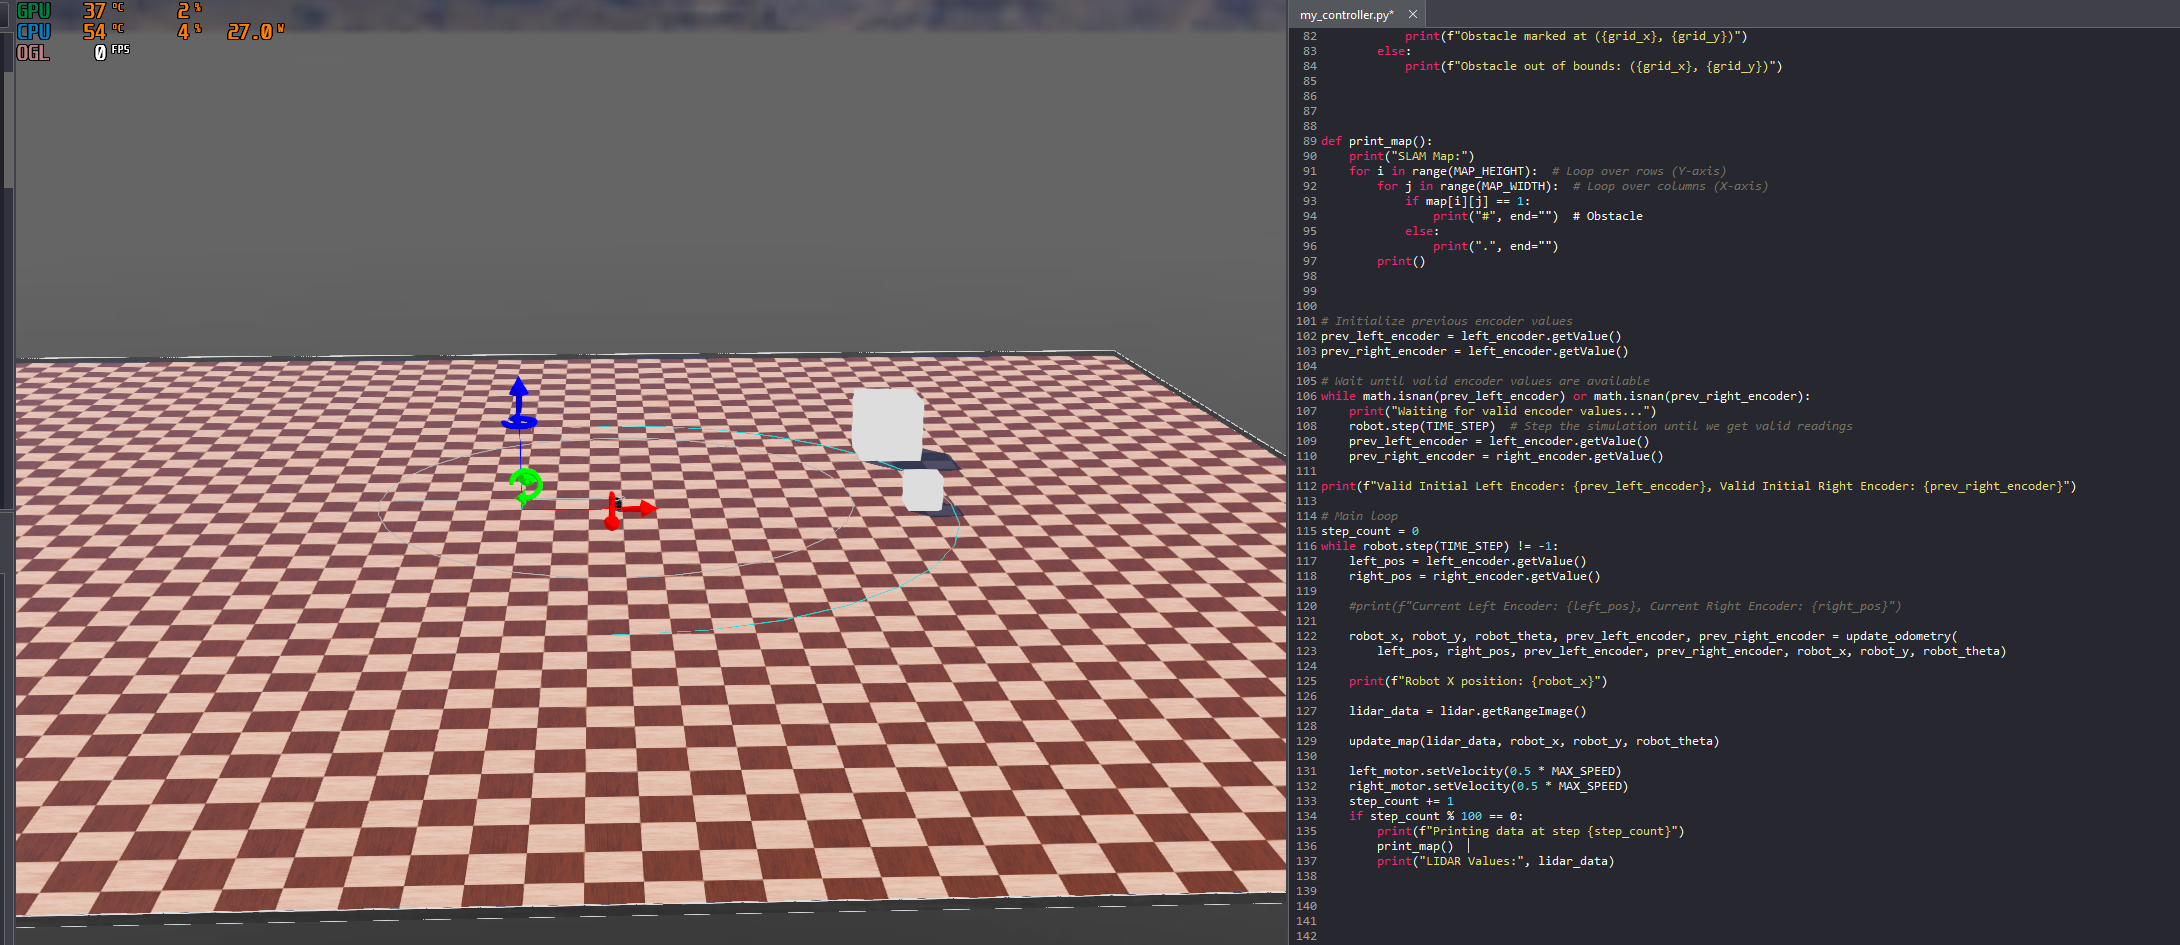
\includegraphics[width=1.0\linewidth]{midpoint_report/assets/images/localisation/slam_arena.png}
    \caption{A basic SLAM Arena in Webots}
    \label{fig: slam_arena image} 
\end{figure}

\begin{figure}[H]
    \centering
    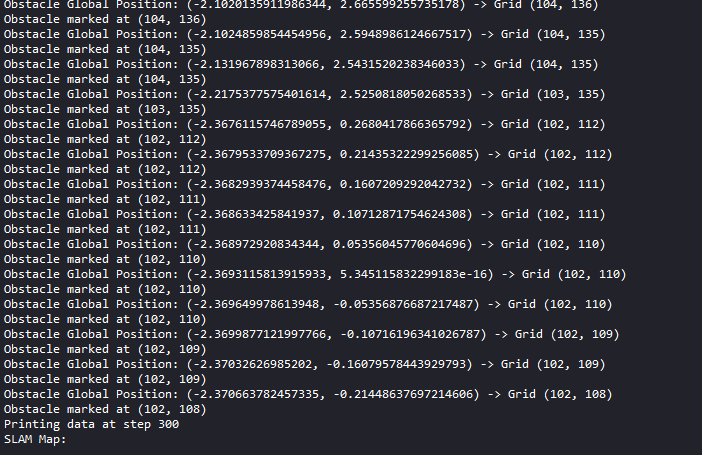
\includegraphics[width=1.0\linewidth]{midpoint_report/assets/images/localisation/coordinates.png}
    \caption{Local and Global coordinates of the Robot}
    \label{fig: coordinates} 
\end{figure}

\begin{figure}[H]
    \centering
    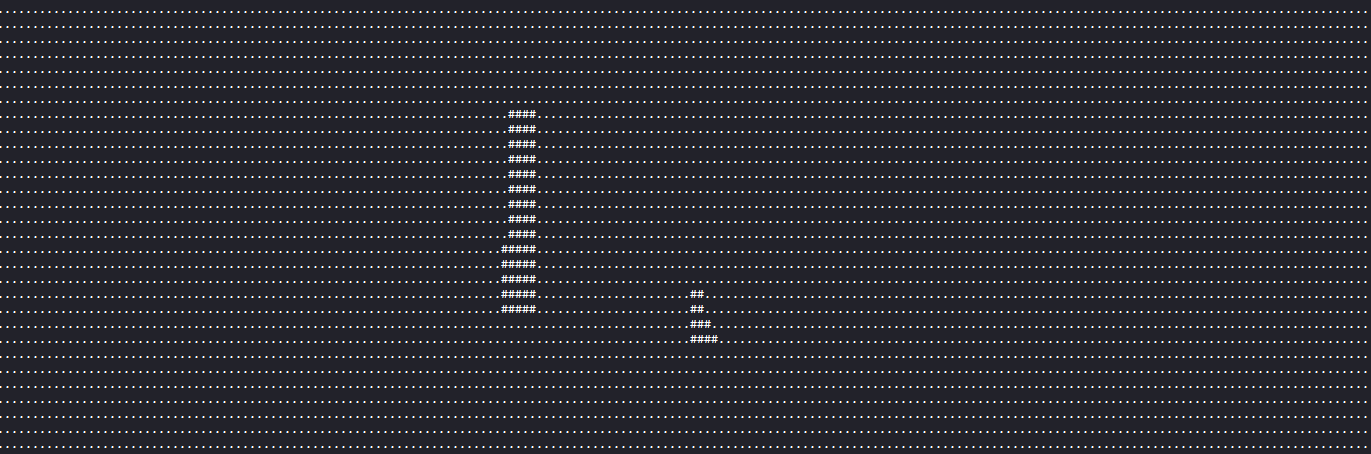
\includegraphics[width=1.0\linewidth]{midpoint_report/assets/images/localisation/map.png}
    \caption{A 2-D map depicting the location of the robot in its environment}
    \label{fig: map} 
\end{figure}



\paragraph*{}
While our initial implementation focused on localization within a predefined map, we later recognized that this did not fulfill the requirements of SLAM, as it lacked the capability to simultaneously map an unknown environment. To address this limitation, we explored various approaches to implement full SLAM. Our first attempt involved using ROS2 with TurtleBot3 Burger integrated into the Webots simulation to access established SLAM libraries like Gmapping and Cartographer. However, challenges with communication between ROS2 and the simulation, stemming from our limited experience, hindered progress. 

\paragraph*{}Subsequently, we opted for a SLAM method independent of ROS, specifically considering EKF SLAM and Graph SLAM. While EKF SLAM initially appeared promising due to its reliance on the Kalman filter, we ultimately selected Graph SLAM for its superior accuracy and robustness. Graph SLAM performs global optimization by maintaining a graph of all robot poses and measurements, allowing efficient correction of accumulated errors, particularly during loop closures when the robot revisits known locations. This was particularly advantageous for our project, as the robots, after placing objects in their designated locations, would return to the main map. Unlike EKF SLAM, which updates only the current pose and relies on linearization, Graph SLAM adjusts the entire trajectory and map, minimizing drift and handling non-linearities effectively. As a result, we finalized our approach with Graph SLAM to ensure a robust and comprehensive implementation. In the proposal, the use of C-SLAM was mentioned. However; we have shifted from that idea as the idea of of collaborative SLAM seems rather redundant when we already have efficient communication between the robots. 
